%
% Authors
% Denis Augsburger
% Piero Steinger
% Thomas Wilde
% Nicolas Mauchle
% 
%
% Version 1.0
%
\documentclass[12pt,a4paper,german]{article}
%
\author{Denis Augsburger, Piero Steinger, Thomas Wilde, Nicolas Mauchle }
%
\usepackage[left=2.5cm,right=2.5cm,bottom=2.5cm,includeheadfoot]{geometry}
\usepackage[pdftex]{graphicx}
\usepackage{babel}
\usepackage[utf8]{inputenc}
\usepackage{fancyhdr}
\usepackage{lastpage}
\usepackage{multirow}
% For Kontext diagram
\usepackage{pdflscape}
\usepackage{longtable}
\usepackage{caption}
%
% Graue Farbe
\usepackage{blindtext} 
\usepackage{framed} 
\usepackage{xcolor} 
\colorlet{shadecolor}{gray!25} 
\usepackage{color}
\input{utils/colors}
%
\usepackage{hyperref}
\hypersetup{
    pdfborder = {0 0 0}
}
 \usepackage{mathpazo}
%Damit man label setzten kann wo man will
\usepackage[all]{hypcap}
\usepackage[stable]{footmisc}
% KOPF UND FUSS ZEILEN
\pagestyle{fancy}
%
\fancyhf[R]{}
\fancyhf[L]{\leftmark}
%
% suppress page number in bottom center:
\cfoot{}
%
\fancyfoot[L]{}
\fancyfoot[R]{Seite \thepage \  von  \pageref{LastPage}}
%
%Linie unten
\renewcommand{\footrulewidth}{0.5pt}
%
\newcommand{\HRule}{\rule{\linewidth}{0.5mm}}
%
% Document
%
\begin{document}
\begin{titlepage}
\begin{center}
\textsc{\LARGE Fachhochschule Nordwestschweiz}\\[1.5cm]
% Title
\HRule \\[0.4cm]
{ \huge \bfseries Portfolio}\\[0.4cm]
\HRule \\[1.5cm]
% Author and supervisor
\begin{minipage}{1.2\textwidth}
\begin{flushleft} \large
\emph{Autor:}\\
Lea Knöll
\newline
\newline
\emph{Dozent:} \\
René Fankhauser
\newline
\newline
\emph{Klasse:} \\
3. Semester\\
%\end{flushright}
\end{flushleft}
\end{minipage}
\vfill
% Bottom of the page
{\large \today}
\end{center}
\end{titlepage}

\newpage
\tableofcontents
\section{Einleitung}
Für die Firma Nutz AG soll eine neue Applikation entwickelt werden, um die Vermietung und Wartung der Fahrzeuge zielgerichteter anzubieten.\\
Zurzeit hat die Firma ca. 200 verschiedene Nutzfahrzeuge. Ihre Kundendatenbank umfasst über 3000 Privat- sowie auch Geschäftskunden.\\
Durch die verschiedenen Standorte, kommt es immer wieder zu unnötigen Fahrzeugverschiebungen. Auch die Wartung der Fahrzeuge wir momentan mit einer Excelliste rapportiert.\\[2ex]
%
Dies soll durch die neue Webapplikation verbessert und vereinfacht werden.\\
Auf den nächsten Seiten werden die Stakeholder nach ihrer Wichtigkeit identifiziert, in Interessengruppen einteilen.\\
Danach werden wir Probleme sowie Widerstände aufzeigen, die im Verlauf des Projektes auftretten könnten.\\
Um an die richtigen Informationen zu gelnagen, zeigen wir für jede Interessegruppe unsere Idee für die \textit{Erhebung der Informtionen} auf.\\
Durch das Kontextdiagramm veranschulichen wir den ganzen Arbeitsprozess\\
Zum Schluss definieren wir noch unsere Ziele, die wir in diesem Projekt erreichen möchten.
\newpage
% Beschreiben der Interessengruppe (Aufgabe 1)
\section{Interessengruppen}
%
Wir haben folgende Interessengruppen gefunden.
\begin{center}
  \begin{figure}[ht]
    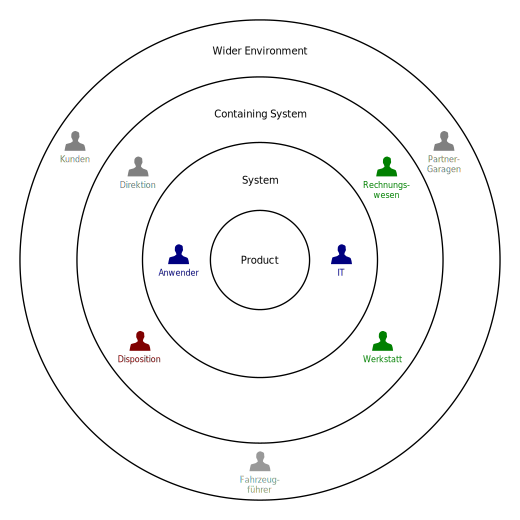
\includegraphics{aufgabe1/graphics/onion.pdf}
    \caption{Onion-Diagramm der Nutz AG Steakholders}
    \label{fig:awesome_image}
  \end{figure}
\end{center}
%
\textbf{Anwender}\\
Die Anwender sind für die Verwaltung des Fahrzeugparks zuständig. Es handelt sich meist um Angestellte mit einem kaufmännischen Hintergrund.Sie möchten mit dem System bestehende Abläufe möglichst einfach ausführen. 
\\[6ex]
%
\textbf{IT}\\
Die IT besteht aus 3 Mitarbeitern im Support. Komplexere Aufgaben werden mit externen Partnern realisiert. Ein AS400-System ist im Einsatz und der Wartungsvertrag läuft in 14 Monaten aus. Dies ist der Endtermin aus Sicht der IT. Der IT-Verantwortliche hat klare Vorstellungen an das neue System, welche teilweise ausserhalb des Einsatzgebietes liegen. Die Software soll umfangreich und trotzdem einfach nutzbar sein. Die Wartungsarbeiten an Serversystemen soll für den Support minimiert werden.
\\[2ex]
\textbf{Rechnungwesen}\\
Das Rechnungswesen möchte die Kosten um 20\% mit dem Projekt senken. Das Berichtswesen soll ausgebaut werden. Die Zahlungsmoral soll verbessert werden, beispielsweise durch eine "realtime" Debitorenbuchhaltung. Ebenfalls soll eine Auswertung der Debitoren nach Kunden, Kundengruppen, Fahrzeugkategorien möglich sein. Diese Auswertung dient den Führungskräften zur Kommunikation gegen Innen und Aussen. Ziel für das Rechnungswesen ist es den Gewinn zu optimieren.
\\[2ex]
\textbf{Disposition}\\
Die Disposition ist verantwortlich, dass sich die Fahrzeuge zum richtigen Zeitpunkt am richtigen Ort befinden. Die interne Organisation ist den Beteiligten klar. Bestehende Arbeitsabläufe sollen möglichst nicht verändert werden, da diese bereits mehrmals optimiert wurden.
\\[2ex]
\textbf{Direktion}\\
Der Direktor hat noch kein konkretes Budget erstellt. Die Obergrenze für das Projekt befindet sich zwischen 600'000 - 800'000 CHF. Er möchte keine Unruhe mit dem Projekt stiften, da er bald in Pension geht.
\\[2ex]
\textbf{Weitere Stakeholder}\\
Die Fahrzeuge dürfen nur im Inland eingesetzt werden. Wir vermuten wegen Versicherungsbedingungen und fehlendem Pannendienst. \\
Die Garagen müssen im Vorfeld über den Einsatz des Mietfahrzeugs in Ihrer Region informiert werden. Diese möchten für entsprechende Pannen im Vorfeld disponieren. \\
Die Kunden erwarten einen reibungslosen Ablauf bei der Miete der Fahrzeuge. Umständliche Formalitäten und lange Wartezeiten sollten möglichst vermieden werden.
\section{Mögliche Widerstände}
  \subsection{Dispositionsabteilung}
  Laut dem Abteilungschef läuft der bestehende Prozess einwandfrei. Es besteht eine Tendenz gegen die Erarbeitung der neuen Plattform.
  Der Firmendirektor meinte, es hätte mehrmals Diskussionen darüber gegeben.\\
  %
  Der Abteilungschef sollte im Informationsfluss mit einbezogen werden. Ziel ist, ihn dennoch von den Vorteilen des neuen Systems zu überzeugen.
  %
  \subsection{Low-Profile}
  Die Direktion wünscht sich eine nicht-zu-invasive Entwicklungsphase, was das Requirement Engineering etwas schwieriger macht.\\
  %
  Mit guter Vorbereitung und wenigen, jedoch gezielten Terminen mit wenigen Personen könnte der "Aufdringlichkeitsfaktor" reduziert werden. 
  %
  \subsection{Projektleitung}
  Der IT-Chef als interner Projektleiter scheint nicht sehr gut qualifiziert zu sein. Dazu steht er unter viel Stress.
\section{Probleme und fehlende Informationen}

% TODO: This is a draft! I have to rewrite it later ;-)
\section{Erhebung der Informationen}
\subsection{Anwender}
Für die Anwender schlagen wir eine Workshop vor. Dieser soll aufzeigen, in welche Richtung das ganze gehn sollte beziehungsweise die zu wünschende Aufgaben des Programms.
%
\subsection{IT}
Bei der IT können wir uns ein Prototyp vorstellen. Die IT kennt das System und weiss wo es hackt und wo man es verbessern könnte. Wir gehen davon aus, dass die IT schon weiss in welche Richtung sie die Webapplikation haben möchte. Hier geht es darum, um zu sehen ob es überhaupt machbar ist. Ein Prototyp würde schön zeigen, wie es sich die IT Vorstellt und die es man kann schon mal ein bisschen einschränken.
%
\subsection{Rechnungswesen}
Hier schlagen wir einen Workshop vor, der die Anwendungsfälle involviert. Wir finden es wichtig, dass wir hier genau sehen, wie sich das ganze abspielt und wo wir mit der Applikation helfen können, ihre Kosten zu senken.
%
\subsection{Disposition}
Die Disposition ist sehr negativ auf unser Projekt eingestimmt. Das müssen wir ändern. Wir finden, mit neuen kreativen Techniken können wir das ändern. Wichtig ist, dass wir ihnen zeigen können, dass sie mitbestimmen können bzw. müssen. 
%
\subsection{Direktion}
Der Direktor hat nicht viel Zeit, deshlab würden wir hier noch ein weiters Interview mit Presentation plannen, um die nächsten Schritte zu besprechen und unsere Informationen, die wir von den Mitarbeiter gesammelt haben, presentieren.\\
Zu diesem Zeitpunkt müssen wir es geschafft haben, die Disposition von dem Projekt zu überzeugen. Was wir aber im Hinterkopf behalten müssen, ist dass der Direktor in ein paar Jahren pensioniert wird. Ihm ist die gemütlichkeit bequemer als dass das Projekt ein Erfolg wird.
%
\subsection{Kunden}
Bei den Kunden würden wir vorschlagen einen Fragebogen zu verwenden. Da es über 3000 Kunden sind, ist das die geeignetste Methode.\\
Es natürlich klar das man hier nie auf alle Kundenwünsche eingehen kann. Aber man kann mit einem guten Fragebogen die Richtung der Kunden herauslesen.
\subsection{Benutzer des Systems}
Wir haben die Nutzer des System in zwei Gruppen aufgeteilt. Die \textbf{Heavy-User}, die User die hauptsächlich mit der Webapplikation arbeiten werden.\\
Daneben haben wir die \textbf{User}. Sie kommen mit der Webapplikation in Berührung, sind aber nicht so stark darauf angewiesen wie die Heavy-User.
%
\subsubsection{Heavy-User}
Die Heavy-User der Webapplikation sind:
\begin{itemize}
\item Die Disposition
\item Die Anwender
\item Das Rechnungswesen
\end{itemize}
%
\subsubsection{User}
Für die Webapplikation haben wir folgende User
\begin{itemize}
\item Die IT-Abteilung
\item Die Werkstatt
\item Der Kunde
\item Die Direktion
\item Fahrzeugführer
\end{itemize}
\subsection{Priorisierung der Stakeholder}
Für uns haben folgende Interessengruppen eine hohe Wichtigkeit.
\begin{itemize}
\item Die Anwender
\item Die IT-Abteilung
\item Die Disposition
\item Das Rechnungswesen
\end{itemize}
%
Sie alle werden viel mit der Webapplikation arbeiten. Sie entscheiden ob das Projekt ein Erfolg ist oder nicht. Dies bedeutet, dass wir ihre Ziele und Wünsche gegenüber anderen Gruppen priorisieren.\\[2ex]
%
Als wichtig erachten wir folgende Interessengruppen.
\begin{itemize}
\item Die Direktion
\item Die Werkstatt
\item Die Kunden
\end{itemize}
%
Da der Direktor nicht mehr lange bei der Firma ist, hat er für uns nicht eine solch hohe Wichtigkeit. Wir müssen ihn nur von unserem Projekt überzeugen. Dies können wir, wenn die oben genannten Interessengruppen hinter dem Projekt stehen. Da nach seiner Ära ein neuer Direktor kommt und andere Ziele oder Wünsche hat, müssen wir mit den Wünschen vorsichtig umgehen.\\[2ex]
%
Nicht so wichtig sehen wir
\begin{itemize}
\item Die Partner Garagen
\item Die Fahrzeugführer
\end{itemize}
%
Die Partner Garagen, sowie die Fahrzeugführer haben mit der neuen Webapplikation praktisch keinen Kontakt. Somit sind sie für dieses Projekt nicht wichtig.\begin{titlepage}
\begin{center}
\textsc{\LARGE Fachhochschule Nordwestschweiz}\\[1.5cm]
% Title
\HRule \\[0.4cm]
{ \huge \bfseries Portfolio}\\[0.4cm]
\HRule \\[1.5cm]
% Author and supervisor
\begin{minipage}{1.2\textwidth}
\begin{flushleft} \large
\emph{Autor:}\\
Lea Knöll
\newline
\newline
\emph{Dozent:} \\
René Fankhauser
\newline
\newline
\emph{Klasse:} \\
3. Semester\\
%\end{flushright}
\end{flushleft}
\end{minipage}
\vfill
% Bottom of the page
{\large \today}
\end{center}
\end{titlepage}


\newpage
% Aufgabe 2 Kontext 
\section{Kontext}
\captionof{table}{Kontextbeschreibung}
  \begin{tabular}{| l | l | l|}
    \hline
    \textbf{Anforderungsquellen} & \textbf{Betrachtungsgegenstände} \\ \hline
    Bestehende Prozesse
    &
    {\parbox{0.7\textwidth}{
      \begin{itemize}
        \item Bestehende Dokumentation der Prozessabläufe.
        \item Dokumentation der bestehenden Software-Lösungen, falls vorhanden.
        \item Datenbankinhalte und Datenformate.
        \item Abteilungsschnittstellen bzw. Kommunkationsmethoden.
        \item Datenfluss bzw. Relevanz der verschiedenen Datenpunkten von einer Abteilung zur nächsten.
        \item Implizite bzw. eingebettete Anforderungen.
      \end{itemize}
    }}
    \\ \hline
    Abteilungsleiter
    &
    {\parbox{0.7\textwidth}{
      \begin{itemize}
        \item Vorstellungen des Endproduktes und dessen Plausibilität 
        \item Kommunikationsmedien, mit welchen die Abteilung arbeitet
        \item Priorisierung der Abläufe d.h. Businesskritische Abläufe zuerst
        \item Abteilungübergreifende Prozesse und dessen Schwachstellen
      \end{itemize}
    }}
    \\ \hline    
    Dokumentation, Fall-Archiv
    &
    {\parbox{0.7\textwidth}{
      \begin{itemize}
        \item Legale Aspekte analysieren; hätte man etwas besser machen können? 
        \item Probleme identifizieren
        \item Nicht vorhandene Dokumentation notieren
      \end{itemize}
    }}
    \\ \hline      
  \end{tabular}

%\begin{landscape}
\begin{center}
  \begin{figure}[ht]
    
\includegraphics[width=\textwidth]{graphics/kontextdiagramm.pdf}
    \caption{Kontextdiagramm des Endproduktes in der Nutz AG}
    \label{fig:awesome_image}
  \end{figure}
\end{center}
%\end{landscape}

\newpage
% Aufgabe 3 Ziele
\section{Ziele mit dem neuen System}
% 7-10 Ziele, messbar, gewichtet, strukturiert, konfliktfrei formuliert
Durch die vorherige Analyse der Anforderungen der Nutzag haben sich unten stehende Ziele ergeben. Diese sind der Reihenfolge nach gewichtet beziehungsweise priorisiert.

\subsection{Ziele der Nutzer}
\begin{enumerate}
\item Alle vermieteten Fahrzeuge werden über das System verwaltet
\item Der administrative Aufwand bei der Vermietung wird um eine Arbeitsstunde pro Tag reduziert
\item Der Kunde erhält sein gewünschtes Fahrzeug zur gewünschten Zeit bei der korrekten Agentur
\item Das System verwaltet den aktuellen Status des Fahrzeuges mit mindestens Vermietung, Reserviert, Wartung, Pannenbehebung und Frei.
\end{enumerate} 
%
\subsection{Ziele weiterer Stakeholder}
\begin{enumerate}
\item Das Projekt kostet weniger als 800'000 CHF
\item Die Software löst bis zum 31. Dezember 2014 das bestehende System ab.
\item Die Kosten für die Disposition der Fahrzeuge soll im Durchschnitt um 20\% gesenkt werden.
\end{enumerate}
\listoffigures
\listoftables

\end{document}
